\documentclass[slidestop,compress,blackandwhite]{beamer}

\usepackage[utf8x]{inputenc}
\usepackage[italian]{babel}
\usepackage{tikz}
\usepackage{nameref}
\usepackage{scrextend}

\usetheme{Antibes}
\usecolortheme{default}


\pgfdeclareimage[height=1.5cm]{logo}{imgs/unipd_logo}

\setbeamercolor{block title}{fg=red,bg=structure!15}

\setbeamercolor{block body}{bg=structure!15}

% TITOLO
\setbeamercovered{transparent}

\author{Moreno Ambrosin}

\title[Progetto esame di Sistemi Concorrenti e Distribuiti]{Railway Simulation}

\institute[\insertframenumber/\inserttotalframenumber]{
	\large{Università degli studi di Padova} \\
	\vspace{5pt}
	\normalsize Facoltà di Scienze MM. FF. NN. \\
	\vspace{5pt}
	\small Corso di laurea in Informatica
}
\date{Settembre 2013}

\newcommand{\itemB}[3]{
	\item \textbf{#1} #2 \vspace{#3}
}

\newcommand{\ttt}[1]{\texttt{#1}}
\newcommand{\ii}[1]{\textit{#1}}

\newcommand{\treno}{\ii{treno}}
\newcommand{\treni}{\ii{treni}}
\newcommand{\viaggiatore}{\ii{viaggiatore}}
\newcommand{\viaggiatori}{\ii{viaggiatori}}
\newcommand{\stazione}{\ii{stazione}}
\newcommand{\stazioni}{\ii{stazioni}}
\newcommand{\piattaforma}{\ii{piattaforma}}
\newcommand{\piattaforme}{\ii{piattaforme}}
\newcommand{\ticket}{\ii{biglietto}}
\newcommand{\tickets}{\ii{biglietti}}
\newcommand{\segmento}{\ii{segmento}}
\newcommand{\segmenti}{\ii{segmenti}}
\newcommand{\route}{\ii{percorso}}
\newcommand{\routes}{\ii{percorsi}}
\newcommand{\stage}{\ii{tappa}}
\newcommand{\stages}{\ii{tappe}}
\newcommand{\biglietteria}{\ii{biglietteria}}
\newcommand{\biglietterie}{\ii{biglietterie}}
\newcommand{\timetable}{\ii{tabella oraria}}
\newcommand{\timetables}{\ii{tabelle di orari}}
\newcommand{\controller}{\ii{controllo centrale}}
\newcommand{\regione}{\ii{regione}}
\newcommand{\regioni}{\ii{regioni}}
\newcommand{\gateway}{\ii{stazione di gateway}}
\newcommand{\gateways}{\ii{stazioni di gateway}}

\newcommand{\PRO}{\textbf{PRO:}}
\newcommand{\CONTRO}{\textbf{CONTRO:}}


\newcommand{\cm}[1]{\vspace{#1cm}}

\newcommand{\describe}[2]{
	\textbf{#1}\\
	\begin{addmargin}[2em]{0em}
		#2
	\end{addmargin}
}


\newcommand{\newtitle}[4]{
	#1 
	\ifx&#2&%
	\else
  		\large- #2
	\fi
	\ifx&#3&%
	\else
  		\normalsize- #3
	\fi
	\ifx&#4&%
	\else
  		\normalsize (#4)
	\fi
}

\newcommand{\newframe}[5]{
	\begin{frame}
		\frametitle{\newtitle{#1}{#2}{#3}{#4}}
		#5
	\end{frame}
}

\newcommand{\itemt}[1]{\item (\ttt{#1})}
\newcommand{\myitemize}[1]{\begin{itemize}#1\end{itemize}}

\begin{document}
	
	\usebackgroundtemplate{
		\hspace{0.13\paperwidth}
\includegraphics[height=\paperheight]{imgs/logoUnipd}
	}	
	
	\begin{frame}[c]
		\titlepage
	\end{frame}
	
%	\logo{\pgfuseimage{logo}}
	
%	\usebackgroundtemplate{}
	
	\begin{frame}
		\frametitle{Indice}
		\tableofcontents
	\end{frame}
	
	\setbeamertemplate{footline}[text line]{\parbox{\linewidth}{\vspace*{-8pt}\scriptsize\insertframenumber/\inserttotalframenumber\hfill Progetto Sistemi Concorrenti e Distribuiti\hfill}}
	
	\section{Il Problema}\label{problem}
	
	\subsection{Descrizione}
	
	\newframe{\nameref{problem}}{Descrizione}{}{}{
		Simulatore software concorrente e distribuito, per la simulazione di un sistema ferroviario composto da:
		\begin{itemize}
			\item \treni, appartenenti a diverse categorie.
			\item \viaggiatori, che operano azioni elementari come acquisto di \tickets, salita a bordo e discesa dai treni, attesa presso la \piattaforma.
			\item \stazioni~composte da 
				\begin{itemize}
					\item \piattaforme~di attesa per i \viaggiatori;
					\item una \biglietteria~interna, accessibile ai \viaggiatori;
					\item un \ii{pannello informativo}.
				\end{itemize}
			\item \segmenti~che collegano le diverse \stazioni.
			\item un \controller~che mantiene lo stato di ciascun \treno~e di ciascun \viaggiatore~in transito.
		\end{itemize}
	}
	
	\subsection{Requisiti di alto livello}\label{requirements}
	
	\newframe{\nameref{problem}}{\nameref{requirements}}{}{1}{
		
		\vspace{0.5cm}
		\textbf{Stazione}
		\begin{itemize}
			\itemt{RST1} Ciascuna \stazione~è caratterizzata da un identificativo univoco.
			\itemt{RST2} Ciascuna \stazione~contiene:
				\begin{itemize}
					\item Un numero $N$ di \piattaforme~a percorrenza bidirezionale e ad accesso mutuamente esclusivo per la sosta dei \treni, e per l'attesa dei \viaggiatori.
					\item Un \ii{pannello informativo} che riporta informazioni su \treni~in arrivo, in transito, e che hanno appena superato la \stazione.
					\item Una biglietteria accessibile ai \viaggiatori, per l'acquisto del \ticket~necessario.
				\end{itemize}
		\end{itemize} 
		
	}
	
	
	\newframe{\nameref{problem}}{\nameref{requirements}}{}{2}{
	
		\vspace{0.5cm}
		\textbf{Segmento}
		\begin{itemize}
			\itemt{RS1} Ciascun \segmento~ha un identificativo univoco, una lunghezza e una velocità massima di percorrenza; esso collega due \stazioni~diverse.
			\itemt{RS2} Un \segmento~ha percorrenza bidirezionale; inoltre più \treni~possono percorrere il \segmento~nello stesso senso di marcia (percorrenza multipla).  
		\end{itemize}
	
	}

	\newframe{\nameref{problem}}{\nameref{requirements}}{}{3}{
		
		\vspace{0.5cm}
		\textbf{Viaggiatore}
		\begin{itemize}
			\itemt{RV1} Ciascun \viaggiatori~possiede una \stazione~di partenza ed una di destinazione.
			\itemt{RV2} Per poter salire a bordo di un \treno, ciascun \viaggiatori~deve prima acquistare un \ticket~presso la \biglietteria~della \stazione~di partenza.
			\itemt{RV3} Una volta arivato a destinazione, ciascun \viaggiatore~attende un tempo casuale prima di ritornare alla stazione di partenza.
			\itemt{RV4} Il viaggio di ciascun \viaggiatore~può comprendere cambi di \treno.
		\end{itemize}
		
	}

	\newframe{\nameref{problem}}{\nameref{requirements}}{}{4}{
		\textbf{Treno}
		\begin{itemize}
			\itemt{RT1} Ciascun \treno, appatiene ad una delle seguenti categorie: \ttt{FB} o \ttt{REG}.
				\begin{itemize}
					\itemt{RT1.1} La categoria \ttt{FB} è a prenotazione. 
					\itemt{RT1.2} La categoria \ttt{FB} ha priorità maggiore rispetto alla categoria \ttt{REG}. 
				\end{itemize}
			\itemt{RT2} Ciascun \treno~è caratterizzato da un identificativo univoco, e possiede capienza e velocità massime, e mantiene stazioni di partenza e destinazione.
			\itemt{RT3} Ciascun \treno~effettua ripetutamente un tragitto di andata e ritorno, definito da un \route~costituito da più \stages.
				\begin{itemize}
					\itemt{RT3.1} Il tragitto di ciascun \treno~è scandito da una \timetable, che definisce,per ciascuna \stage, l'orario di partenza.
%				\end{itemize}
%		\end{itemize}
%		\begin{itemize}
%			\item[]
%			\begin{itemize} 
				\itemt{RT3.2} Ciascuna \stage~definisce:
				\begin{itemize}
					\item \stazioni~di partenza e destinazione
					\item \piattaforme~di partenza e destinazione
					\item azione da compiere all'arrivo presso la destinazione, tra \ttt{STOP} e \ttt{PASS}
					\item il prossimo \segmento~da utilizzare.
				\end{itemize}
			\end{itemize}
			\itemt{RT4} I \treni~di tipo \ttt{FB} sono a prenotazione.
		\end{itemize}
	}


	
	\subsection{Entità di Simulazione}\label{entities}

	\newframe{\nameref{problem}}{\nameref{entities}}{}{}{
		Indipendenti dalle scelte di distribuzione.
		
		\vspace{0.2cm}
		\describe{Treno}{Entità \ii{attiva}.}
	
		\describe{Viaggiatore}{Entità \ii{attiva}.}
		
		\describe{Segmento}{Entità \ii{reattiva} con agente di controllo, a molteplicità $N>1$.}
		
		\describe{Piattaforma}{Entità \ii{reattiva} con agente di controllo, a molteplicità $1$.}
		
		\describe{Stazione}{Struttura dati che contiene $n\ge1$ \piattaforme, una \biglietteria~e un \ii{pannello informativo}. Fornisce un'interfaccia per l'interazione con \piattaforme~e \biglietteria.}
	}


%###################################### DISTRIBUZIONE	
\section{Distribuzione}\label{distr}

	\subsection{Caratteristiche desiderabili}\label{characteristics}
	\newframe{\nameref{distr}}{\nameref{characteristics}}{}{}{
		\vspace{0.5cm}
		\begin{itemize}
			\itemB{Distribution Transparency}{}{0.6cm}
			\itemB{Scalabilità}{}{0.6cm} 
			\itemB{Roubustezza ai fallimenti}{}{0.6cm} 
			\itemB{Avvio Ordinato}{}{0.6cm} 
			\itemB{Terminazione in stato Consitente}{}{0.6cm}
		\end{itemize}
	}
	
		
%	\newframe{\nameref{characteristics}}{Distribution Transparency}{}{}{
%		
%		Il sistema appare all'utilizzatore come un sistema monolitico.
%		\begin{itemize}
%			\item Unico metodo per accedere alle risorse (\ii{Access Transparency}).
%			\item Locazione fisica delle risorse (\ii{Location Transparency}) e la loro migrazione (\ii{Migration Transparency}) nascoste.
%			\item Sistema trasparente rispetto a replicazione delle risorse (\ii{Replication Transparency}).
%			\item Sistema trasparente rispetto ad accesso concorrente ad una risorsa condivisa (\ii{Concurrency Transparency}).
%			\item Sistema trasparente rispetto ai malfunzionamenti (\ii{Faliure Transparency}).
%		\end{itemize}
%		
%		Il grado di trasparenza da adottare dipende dal problema.
%	}
%	
%	
%	\newframe{\nameref{characteristics}}{Scalabilità}{}{}{
%		TODO...
%	}

%	
%	\newframe{\nameref{characteristics}}{Avvio Ordinato}{}{}{
%		TODO...
%	}
%	
%	
%	\newframe{\nameref{characteristics}}{Terminazione Consitente}{}{}{
%		TODO...
%	}
	
	\subsection{Scelte progettuali}\label{scelte}
	
	\newframe{\nameref{distr}}{\nameref{scelte}}{}{}{
		
		\begin{itemize}
			\item Criteri di distribuzione.
				\myitemize{
					\item Individuazione delle componenti da distribuire.
				}
			\item Analisi di più soluzioni possibili.
				\myitemize{
					\item Valutazione di aspetti positivi e negativi
				}
			\item Modalità di comunicazione tra le componenti distribuite.
		\end{itemize}
		
		
	}
	
	\subsection{Soluzione A}\label{sol_a}
	
%	\newframe{Soluzione A}{Descrizione}{}{1}{
%		Prima Soluzione valutata: tutte le entità risiedono su un diverso nodo di calcolo.
%		\begin{itemize}
%			\item Ciascuna \stazione, \treno~e \viaggiatore~esegue su uno specifico nodo di calcolo.  
%			\item Le \stazioni~espongono un'interfaccia remota per l'iterazione con \treni~e \vi43aggiatori.
%			\item Unica entità \biglietteria, accessibile ai \viaggiatori~tramite interfaccia esposta dalle \stazioni.
%			\item Unice entità di \controller, che espone interfaccia remota a \treni~e \stazioni.
%			\item Server dei nomi presso il quale le entità si registrano all'avvio del sistema.
%		\end{itemize}
%	}
	
	\newframe{\nameref{distr}}{\nameref{sol_a}}{Descrizione}{}{
		\begin{figure}
			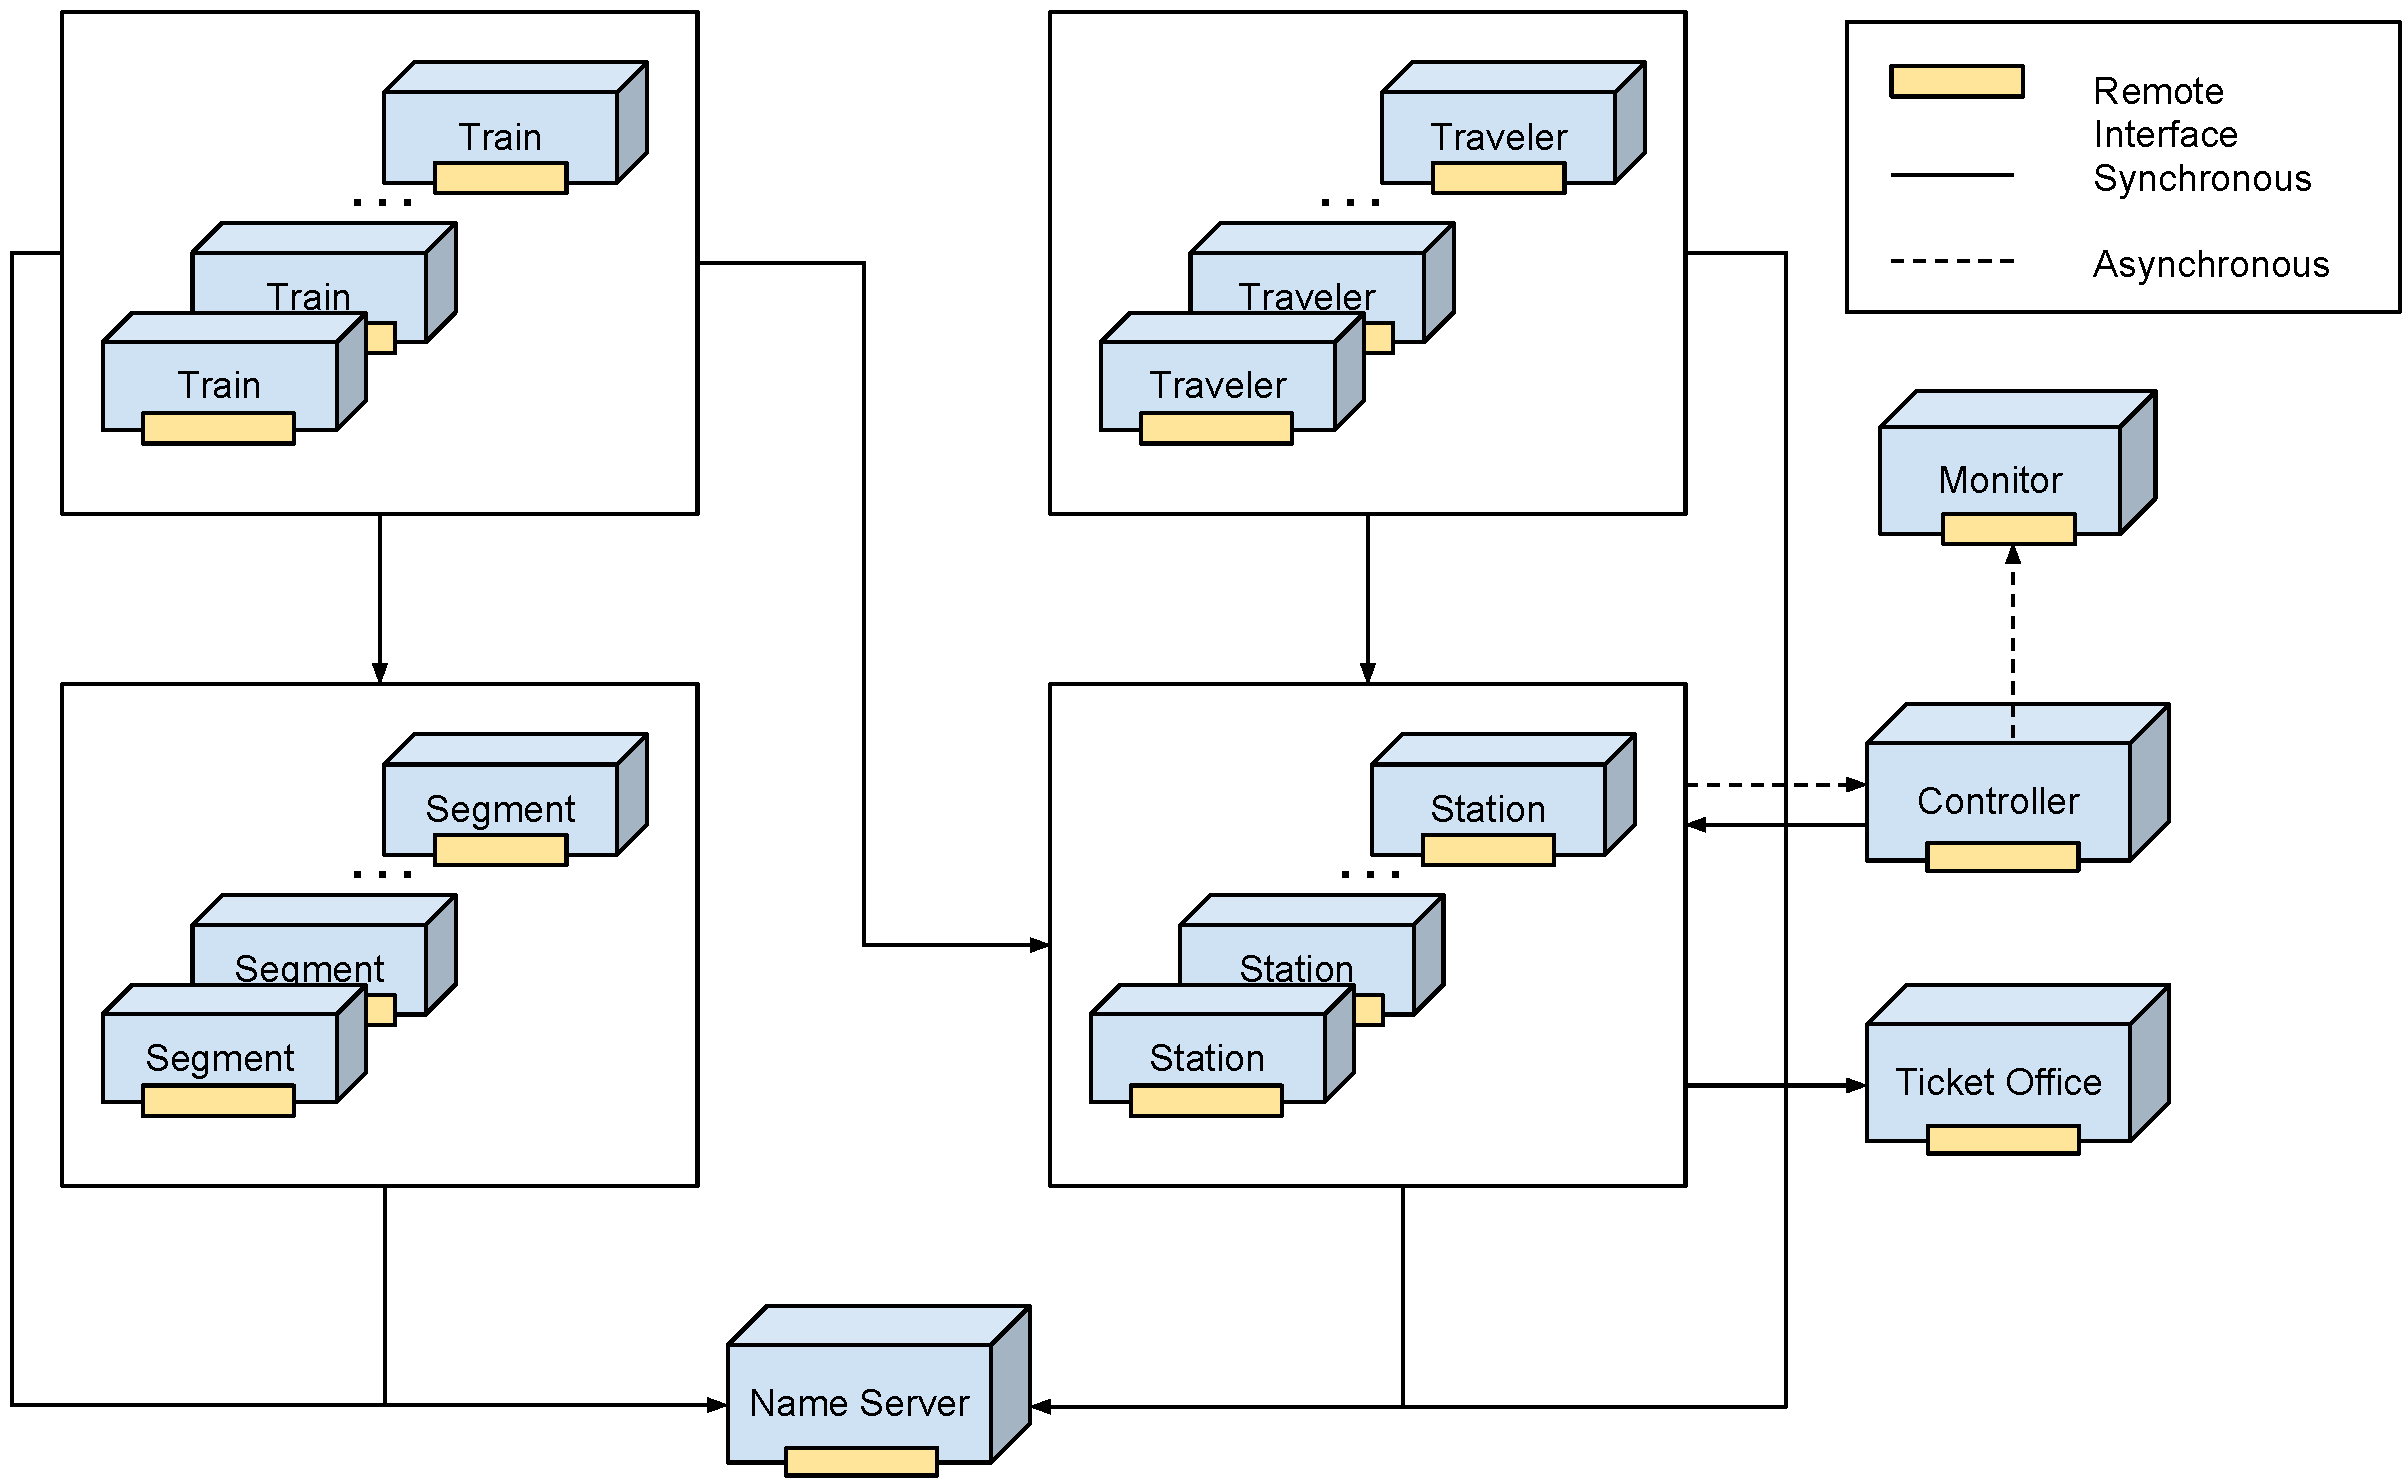
\includegraphics[scale=0.24,trim=0mm 5mm 0mm 35mm]{imgs/All_distributed.pdf}
			\caption{\scriptsize Grafico informale che illustra l'architettura di distribuzione di massima per la Soluzione A; tutte le entità sono distribuite.}
		\end{figure}
	}
	
			
	
	\newframe{\nameref{distr}}{\nameref{sol_a}}{Valutazione}{1}{
		\PRO
			\vspace{0.5cm}
			\begin{itemize}
				\item Sistema scalabile in dimensione rispetto a \treni, \stazioni~e \viaggiatori.
				\vspace{0.5cm}
				\item Robusto rispetto a fallimenti HW e SW a livello di \treni, \stazioni~e \viaggiatori, con impatto ridotto sull'intero sistema.
				\vspace{0.5cm}
				\item \ii{Distribution Transparency} rispetto alle entità \ii{Monitor}.
			\end{itemize}
		
	}

	\newframe{\nameref{distr}}{\nameref{sol_a}}{Valutazione}{2}{
		\CONTRO
			\begin{itemize}
				\item Sincronizzazione in distribuito.
				\item Differenza tra i clock fisici delle macchine che compongono il sistema possono creare inconsistenze.
				\item La \biglietteria~deve mantenere tutta l'informazione relativa alla topologia del sistema ferroviario, e allo stato di prenotazione dei \treni.
				\item Rischio di comunicazioni errate, a causa dell'inaffidabilità della rete; conseguente perdita di performance. 
				\item Elevato traffico di rete al crescere della topologia.
				\item Operazioni di terminazione e avvio del sistema complesse.
			\end{itemize}
	}
	
	\subsection{Soluzione B}\label{sol_b}
	\newframe{\nameref{distr}}{\nameref{sol_b}}{Descrizione}{}{
		\begin{figure}
			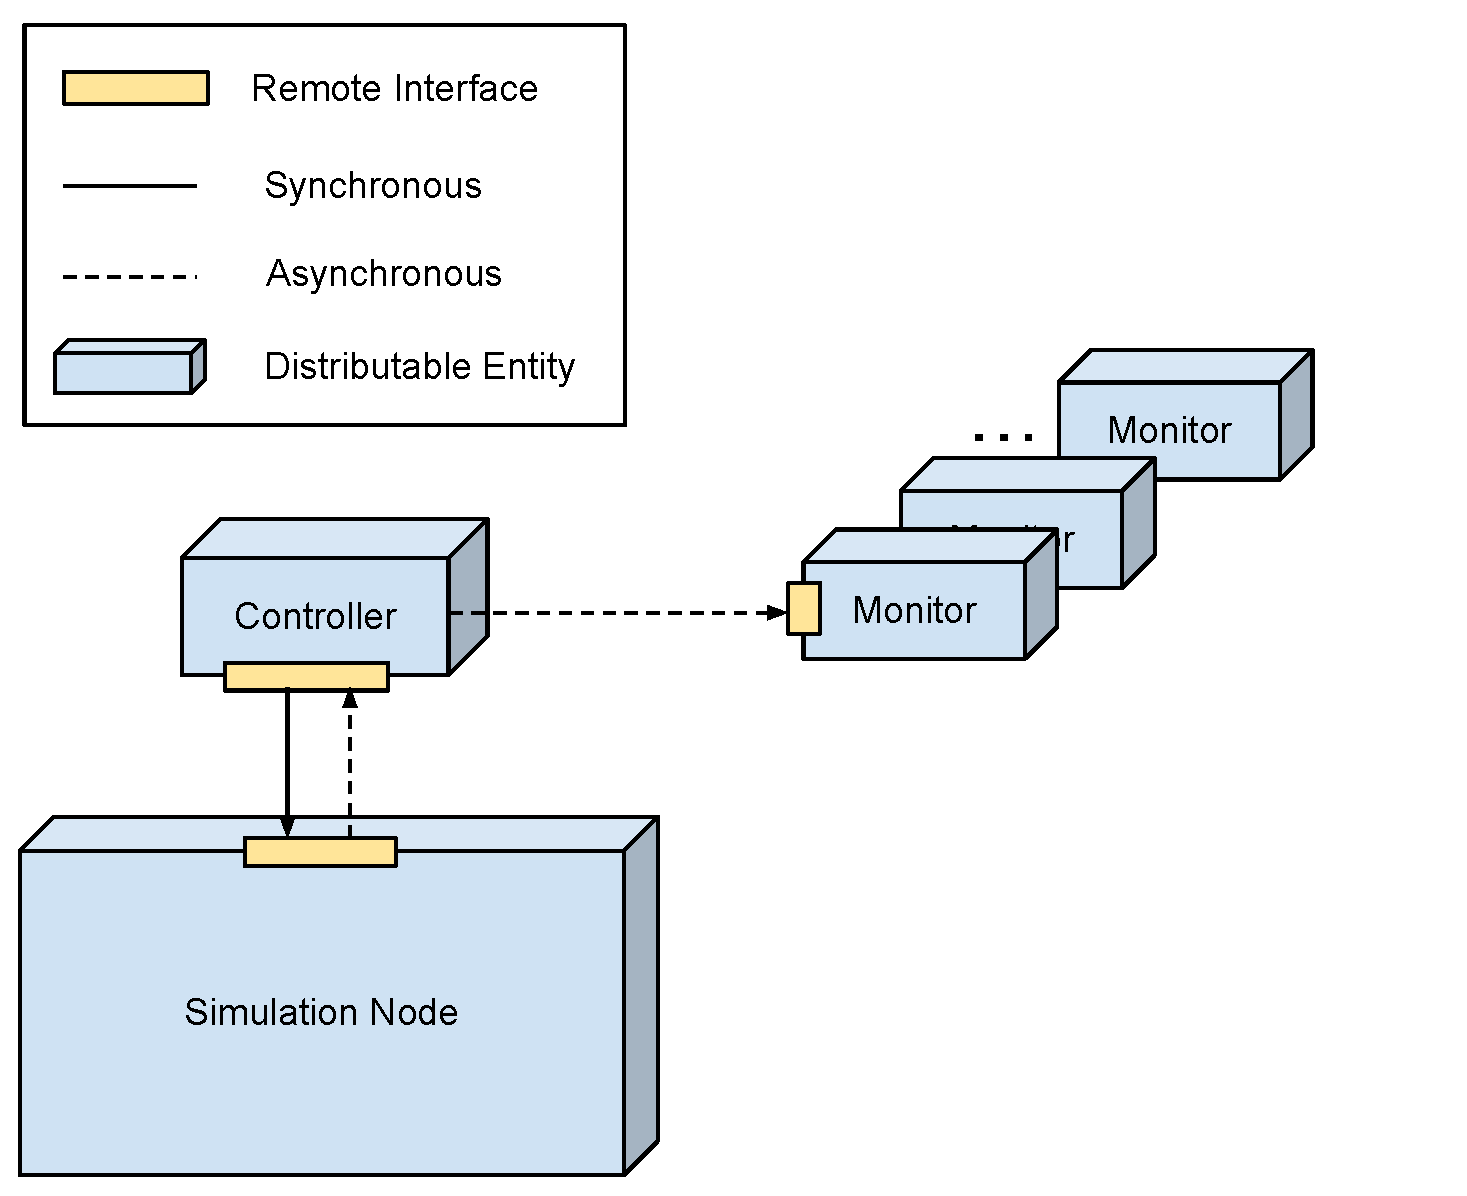
\includegraphics[scale=0.22,trim=0mm 0mm 0mm 0mm]{imgs/nothing_distributed.pdf}
			\caption{\small Grafico informale che illustra l'architettura di distribuzione di massima della Soluzione B; solo \controller~e componente di visualizzazione (\ii{monitor}) sono distribuite.}
		\end{figure}
		
	}
	
	\newframe{\nameref{distr}}{\nameref{sol_b}}{Valutazione}{1}{
		\vspace{0.5cm}
		\PRO
			\begin{itemize}
				\item Seplicità implementativa.
				\item Interazione tra entità risolta in locale mediante meccanismi di concorrenza.
				\item Utilizzo di un unico riferimento temporale; assenza di inconsistenze dovute a clock fisici non sincronizzati.
				\item Semplicità di Avvio e Terminazione dell'intero sistema.
				\item Comunicazione tra le entità di simulazione affidabili.
				\item Traffico di rete minimo.
			\end{itemize}
	}
	
	
	\newframe{\nameref{distr}}{\nameref{sol_b}}{Valutazione}{2}{
		\cm{0.5}
		\CONTRO
			\begin{itemize}
				\item Di scarso interesse.
				\item Fragile rispetto a fallimenti HW e SW, che hanno grande impatto sull'intero sistema.
				\item Non scalabile.
				\item Conoscenza su Topologia e Stato in un unico luogo.
				\item Carico computazionele elevato sul singolo nodo di simulazione.
			\end{itemize}
	}
	

\section{Concorrenza}\label{concurrency}

	\subsection{Caratteristiche Desiderabili}
	\newframe{\nameref{concurrency}}{Caratteristiche Desiderabili}{}{}{
		\cm{0.5}
		\myitemize{
			\item La progettazione deve essere il più possibile indipendente dalle tecnologie.
			\cm{0.5}
			\item La scelta del modello di concorrenza è legata alla natura del problema e alle scelte di distribuzione.
			\cm{0.5}
			\item La soluzione ai problemi di concorrenza deve evitare situazioni di \ii{stallo} o di \ii{starvation}.
		}
	}
	
		\newframe{\nameref{concurrency}}{Vincoli}{}{1}{
		
		\begin{columns}[c]
		\column{0.5\textwidth}
		\begin{enumerate}
			\item Vincoli di accesso ad un \segmento:
				\myitemize{
					\item accesso concorrente tra le entità \treno~intendono accedervi in entrambi i sensi di marcia;
					\item percorrenza multipla in un unico senso di marcia;
					\item mantenimento dell'ordine di accesso;
					\item simulazione della percorrenza dei \treni.
					\item priorità ai \treni~di tipo \ttt{FB}.
				}
		\end{enumerate}
		\column{0.5\textwidth}
		\begin{figure}
			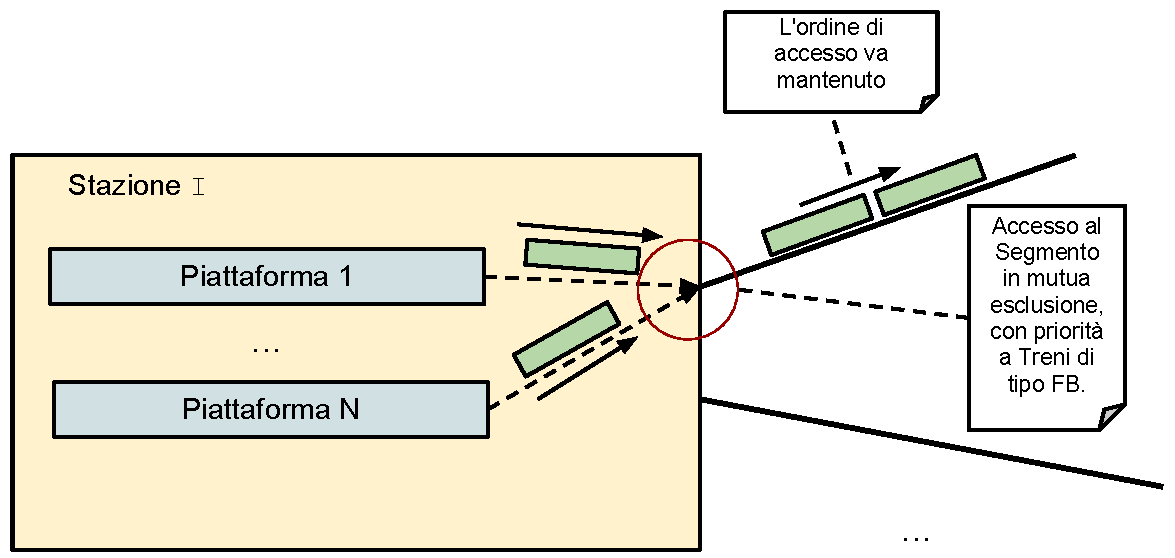
\includegraphics[scale=0.26,trim=0mm 5mm 0mm 35mm]{imgs/ingresso_segmento.pdf}
			%\caption{\scriptsize Grafico informale che illustra l'architettura di distribuzione di massima per la Soluzione A; tutte le entità sono distribuite.}
		\end{figure}
		\end{columns}
	}
	
	\newframe{\nameref{concurrency}}{Vincoli}{}{2}{
		\begin{columns}[c]
		\column{0.6\textwidth}
		\begin{enumerate}
			\setcounter{enumi}{1}
			\item Vincoli di uscita da un \segmento:
				\myitemize{
					\item uscita ordinata dei \treni~in transito secondo l'ordine di accesso.
				}
			\item Vincoli di Accesso ad una \piattaforma:
				\myitemize{
					\item accesso in mutua esclusione, ordinato rispetto ai \treni~provenienti dallo stesso \segmento;
					\item accesso in mutua esclusione, concorente rispetto a \treni~provenienti da \segmenti~diversi;
					\item priorità ai \treni~di tipo \ttt{FB}.
				}
		\end{enumerate}
		\column{0.5\textwidth}
		\begin{figure}
			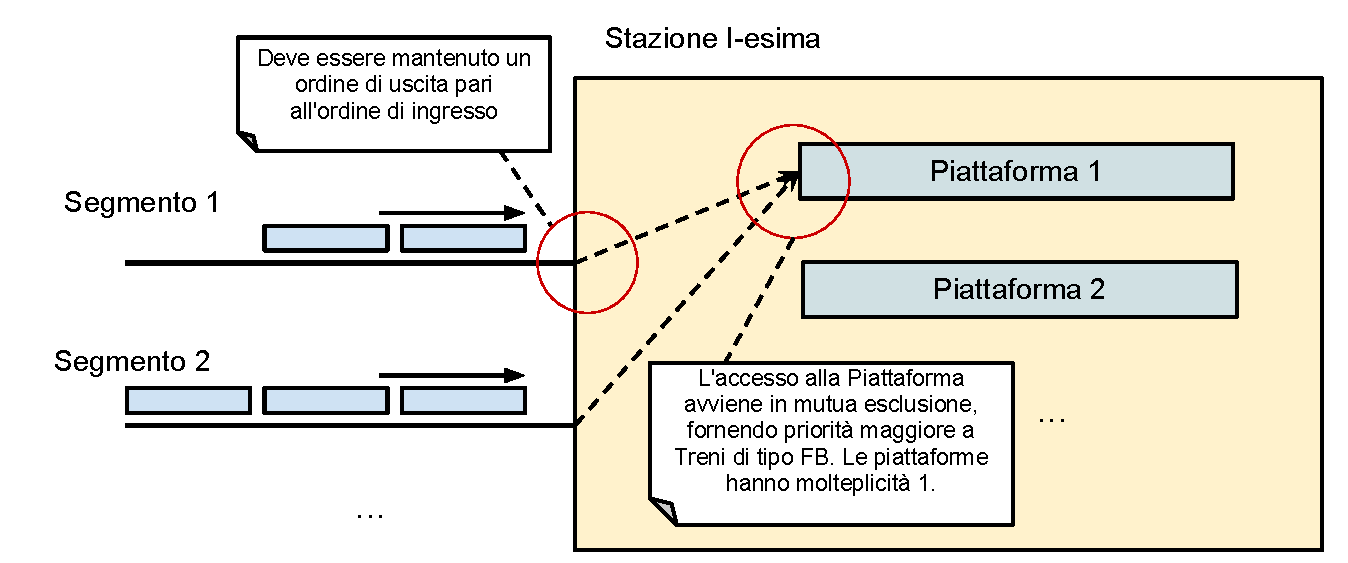
\includegraphics[scale=0.27,trim=30mm 0mm 0mm 0mm]{imgs/Ingresso_Stazione.pdf}
			%\caption{\scriptsize Grafico informale che illustra l'architettura di distribuzione di massima per la Soluzione A; tutte le entità sono distribuite.}
		\end{figure}
		\end{columns}
	}
	
	

% ################################################## SOLUTION ###################################################
\section{Soluzione Adottata}\label{sol}
	
	\subsection{Distribuzione}\label{sol_distr}
	
	\newframe{\nameref{sol}}{\nameref{sol_distr}}{Descrizione}{1}{
		\vspace{0.5cm}
		\begin{itemize}
			\item Soluzione intermedia che mitiga le problematiche riscontrate nelle Soluzioni A e B.
			\item Introduzione di \regioni~per distribuire il carico computazionale su nodi diversi
			\item Ciascuna \regione~è composta da un insieme di \stazioni e di \segmenti, e contiene \treni~e \viaggiatori.
			\item Ciascuna \regione~risiede su un proprio nodo di calcolo.
			\item \`E necessario l'utilizzo di un \ii{Server dei Nomi} per lookup degli indirizzi delle varie \regioni.
		\end{itemize}
	
	}
	
	\newframe{\nameref{sol}}{\nameref{sol_distr}}{Descrizione}{2}{
		\vspace{0.5cm}
		\myitemize{
			\item Introduzione di più livelli di \biglietterie:
				\myitemize{
					\item \ii{interne alle stazioni:} Forniscono da interfaccia per accedere alle biglietterie regionali.
					\item \ii{regionali:} Hanno conoscenza della topologia interna a ciascuna regione; si occupano della creazione dei \tickets.
					\item \ii{centrale:} Mantiene lo stato di prenotazione dei \treni~\ttt{FB} e coordina le creazione di \tickets~interregionali.
				}
			\item L'entità di \controller~è centralizzata, e raccoglie lo stato della simulazione; esso si occupa inoltre delle procedure di Avvio e Terminazione del sistema.
		}
	}
	
	\newframe{\nameref{sol}}{\nameref{sol_distr}}{Descrizione}{3}{
	\begin{figure}
			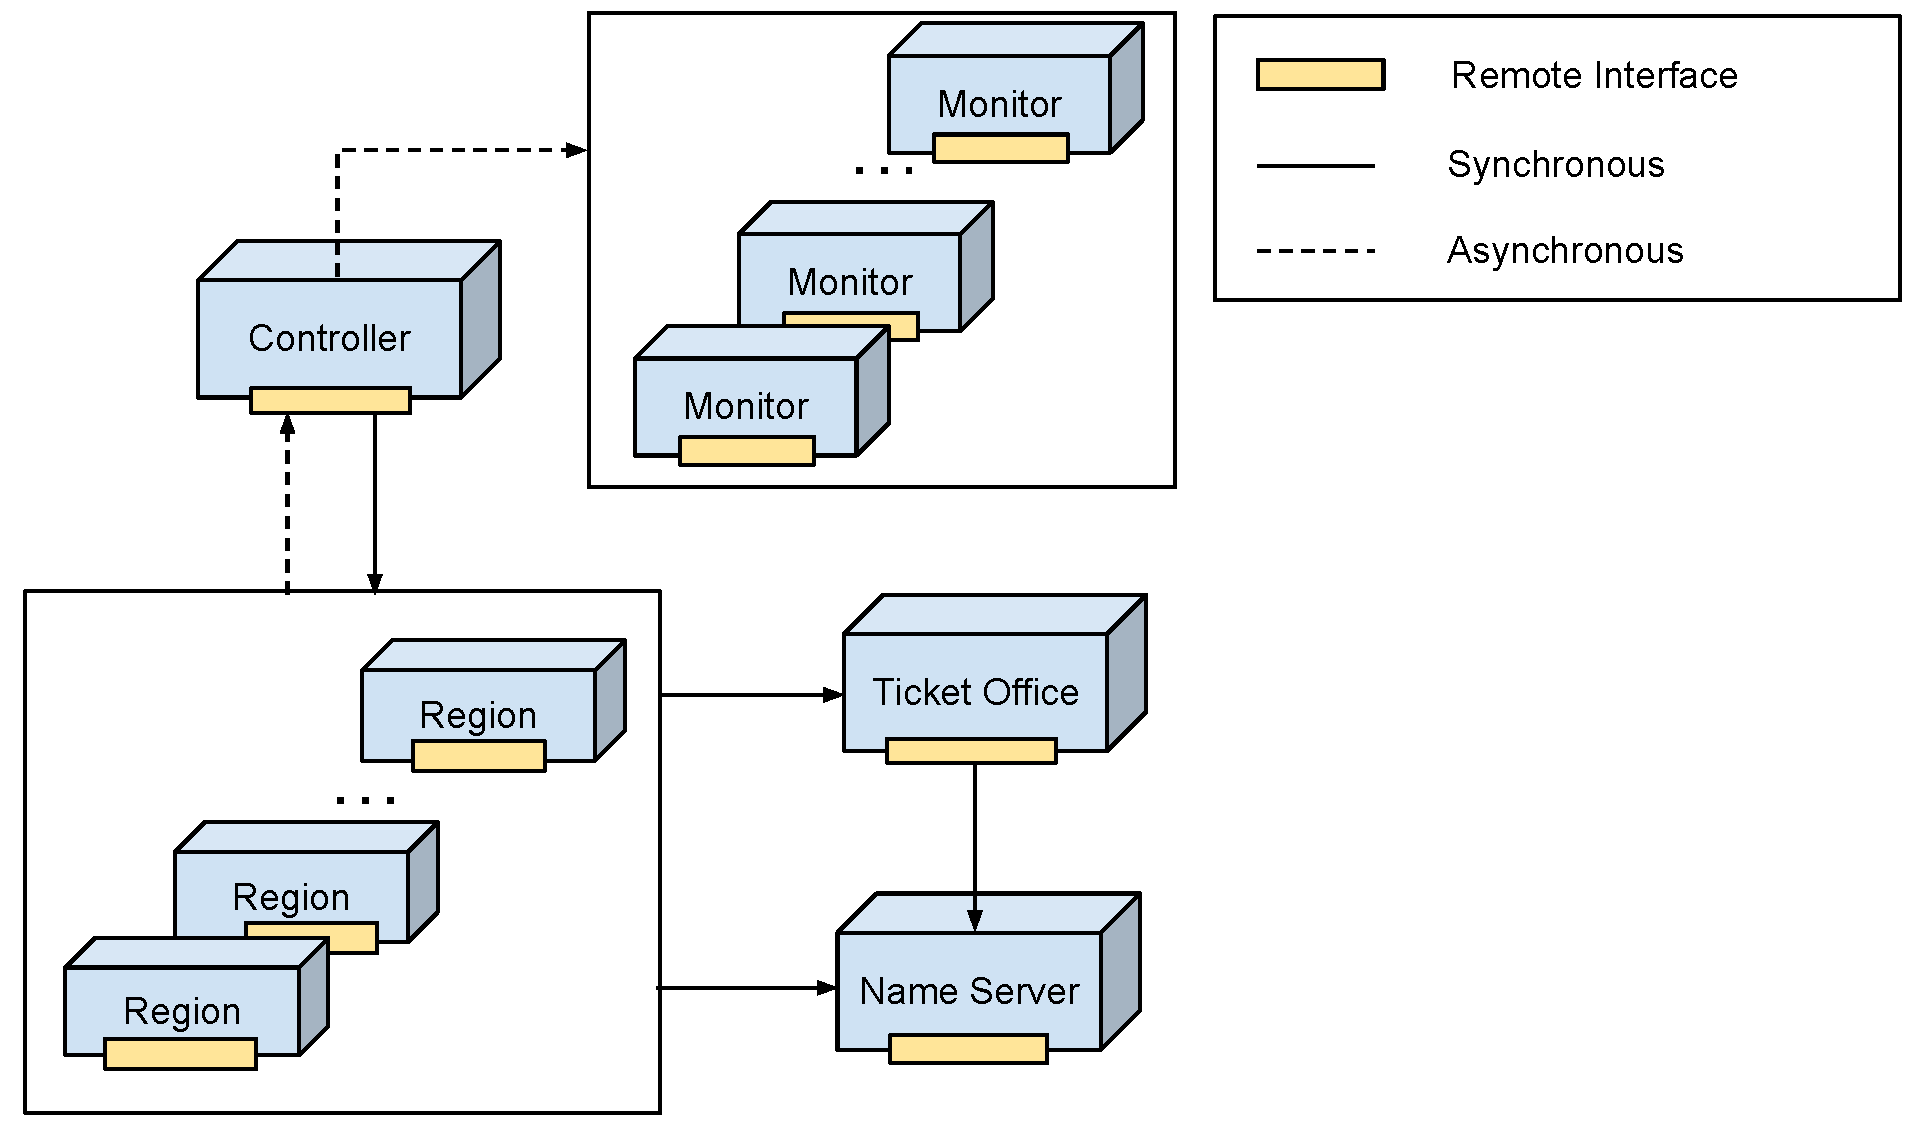
\includegraphics[scale=0.28,trim=0mm 0mm 0mm 20mm]{imgs/solution.pdf}
			\caption{\small Grafico informale che illustra l'architettura di distribuzione di massima dellalla Soluzione presentata.}
		\end{figure}
	}
	
	\newframe{\nameref{sol}}{\nameref{sol_distr}}{Valutazione}{1}{
		\vspace{0.5cm}
		\PRO
		\begin{itemize}
			\item L'utilizzo delle \regioni~è un buon compromesso per controllare la complessità del sistema.
			\item Il sistema è scalabile rispetto alla dimensione.
			\item Distribuisce la conoscenza relativa alla topologia del sistema ferroviario a livello di regioni (non più centralizzata).
			\item La \biglietteria~centrale mantiene solo lo stato relativo alle prenotazioni dei \treni~\ttt{FB}.
		\end{itemize}
	
	}
	
	\newframe{\nameref{sol}}{\nameref{sol_distr}}{Valutazione}{2}{
		\vspace{0.5cm}
		\CONTRO
		\begin{itemize}
			\item Rimane il problema dei clock fisici non sincronizzati, anche se con impatto minore rispetto alla Soluzione A.
			\item Maggiore complessità di Avvio e Terminazione del sistema rispetto alla Soluzione B.
			\item Meno robusta ai fallimenti HW e SW, rispetto alla Soluzione A .
			\item Maggiore traffico di rete rispetto alla Soluzione B
		\end{itemize}
	}
	
	\newframe{Soluzione Adottata}{Requisiti Aggiuntivi}{}{}{
		\cm{0.5}
		\textbf{Requisiti aggiuntivi}
		\cm{0.5}
		\begin{itemize}
			\itemt{RT5} I \treni~possono compiere tragitti che attraversano più \regioni.
			\cm{0.5}	
			\itemt{RV5} I \viaggiatori~possono viaggiare attreverso più \regioni.
		\end{itemize}
	}
	
	\subsection{Problematiche}
	\newframe{Soluzione Adottata}{Problematiche}{}{}{
		\vspace{0.5cm}
		\begin{enumerate}
			\item Come viene effettuato il passaggio di un \treno~tra due \regioni? 
			\vspace{0.4cm}
			\item Come rappresentare il trasferimento di \treni~e \viaggiatori~tra i nodi? 
			\vspace{0.4cm}
			\item Come gestire le problematiche relative al tempo?
%			\vspace{0.4cm}
%			\item Come organizzare avvio e terminazione del sistema?
		\end{enumerate}
	}
	
	\newframe{Soluzione Adottata}{Problematiche}{Passaggio tra regioni}{1}{
		\vspace{0.5cm}
		\myitemize{
			\item Introduzione di \gateways.
			\vspace{0.3cm}
			\item \stazioni~attreverso le quali i \treni~possono uscire dalla \regione~corrente.
			\vspace{0.3cm}
			\item Una volta che un \treno~accede ad una \gateway~presso la \regione~$R$, e viene trasferito su una \regione~$R'$, esso riprenderà il suo \route~dalla \gateway~corrispondente presso $R'$. 
			\item Analogia con i \ii{gateways} di rete.
		}
	}
	
	\newframe{Soluzione Adottata}{Problematiche}{Passaggio tra regioni}{2}{
		\vspace{0.5cm}
		\myitemize{
			\item Sono posti i seguenti vincoli sull'utilizzo di \gateways:
				\myitemize{
					%\item Siano $g$ ed $g'$ \gateways~appartenenti rispettivamente a due \regioni~$R$ ed $R'$. Allora se da $g$ è possibile raggiungere $g'$ in modo diretto (e viceversa), allora $!\exists g''$ appartenente a $R$ tale per cui da $g''$ si può raggiungere $g'$.\\
					%$\Rightarrow$ In questo modo, dal punto di vista dei \treni, $g$ e $g'$ saranno la stessa \stazione~logica.
					\item Se la \regione~$R'$ è raggiungibile dalla \regione~$R$, allora esiste un'unica \gateway~$\in R$ che permette di raggiungere $R'$
					\item \gateways~appartenenti a \regioni~diverse collegate sono considerate a livello logico come un'unica \stazione.
				
				}
		}
	}
	
	
	\newframe{Soluzione Adottata}{Problematiche}{Trasferimento remoto}{1}{
		\myitemize{
			\item Il passaggio di un \treno~( o di un \viaggiatore) da una \regione~ad un'altra, prevede l'interruzione dell'esecuzione dell'entità nel nodo di partenza e la continuazione della stessa nel nodo di destinazione.
			\item Come è opportuno mappare ciascuna entità attiva?
				\myitemize{
					\item Se a ciascun \treno~(\viaggiatore) viene associato ad un thread allora:
						\myitemize{
							\item Il trasferimento può essere ottenuto con distruzione e creazione dei thread associati a \treni~e \viaggiatori~$\Rightarrow$ operazione costosa, preferibilmente da eseguire solo all'avvio del sistema.
							\item Replicazione e attivazione-disattivazione dei thread rispettivamente nei nodi di destinazione e di partenza $\Rightarrow$ Soluzione non scalabile in termini di dimensione della popolazione, e onerosa in termini di risorse utilizzate. 
						} 
				}
		}
	}
	
	\newframe{Soluzione Adottata}{Problematiche}{Trasferimento remoto}{2}{
		\myitemize{
			\item Necessario disaccoppiare le Entità e le operazioni da eseguire, dai thread che le eseguono.
				\myitemize{
					\item In questo modo si trasferiscono solo le informazioni relative all'entità da eseguire (non i thread).
					\item I dati di ciascuna entità sono replicati in tutti i nodi di simulazione, e solamente aggiornati nel momento del trasferimento.	
				}
		}
		\describe{Viaggiatore}{
			\myitemize{
				\item Definito come:
					\myitemize{
						\item Descrittore, che contiene i dati relativi al \viaggiatore;
						\item Insieme di \ii{operazioni} da eseguire su di esso.
					}
				\item \ii{operazioni} eseguite da una struttura composta da un \ii{thread pool} a dimensione statica, e da una coda FIFO di operazioni.
				\item Per eseguire la prossima operazione, essa viene inserita nella coda\\
				$\Rightarrow$ trasferimento del \viaggiatore~realizzato con aggiornamento dei dati relativi al \viaggiatore~e inserimento della prossima \ii{operazione} da eseguire nella coda di operazioni, del nodo destinazione. 
			}
		}
		
		
	}
	
	\newframe{Soluzione Adottata}{Problematiche}{Trasferimento remoto}{3}{
		\describe{Treno}{
			\myitemize{
				\item Ciascun \treno~è rappresentato da un \ii{descrittore}, che contiene i dati che lo caratterizzano.
				\item Viene utilizzata una struttura composta da un \ii{thread pool} a dimensione statica, e da una coda FIFO di \ii{descrittori}.\\
				\item Ciascun thread del pool esegue una sequenza fissata di operazioni per il prossimo \treno~estratto dalla coda di \ii{descrittori}.\\
				$\Rightarrow$ trasferimento di un \treno~realizzato con aggiornamento dei dati relativi al \treno~e inserimento del \ii{descrittore} nella coda apposita, presso al nodo destinazione.
			}
		}
		
	}
	
	\newframe{Soluzione Adottata}{Problematiche}{Trasferimento remoto}{4}{
		\textbf{Problema:} Come dimensionare il \ii{thread pool}?
		\myitemize{
			\item Dipende dai protocolli logici di interazione tra entità attive e reattive;
			\item Scelta tra dimensione \ii{statica} o \ii{dinamica}.
		}
	}
	
	\newframe{Soluzione Adottata}{Problematiche}{Consitenza Temporale}{}{
		\myitemize{
			\item La differenza tra gli orologi fisici delle macchine che compongono il sistema e il ritardo di rete possono generare inconsistenze, in riferimento ai \treni.
%			\item es: un \treno~arriva presso una piattaforma di una \gateway~in orario, al tempo $t$, e dopo il trasferimento si aggiunge un ritardo $\Delta t$.
			\item Adottando \ii{tabelle orarie} che definiscono solo orari di partenza:
				\myitemize{
					\item I ritardi di rete (o dovuti al clock fisico) sono considerati come ritardi dei \treni~della simualzione
					\item Se il clock del nodo destinazione è in anticipo rispetto al clock del nodo do partenza, allora il \treno~trasferito viene considerato in anticipo (può prolungare la sua attesa).
				}
			\item Le differenze vengono accettate.
		}
	}
	
	\subsection{Concorrenza}\label{sol_conc}
	
	\newframe{Soluzione Adottata}{\nameref{sol_conc}}{Scelte Implementative}{}{
		\myitemize{
			\item Scelta del modello di concorrenza da utilizzare.
			\item Valutazione di modelli differenti:
				\myitemize{
					\item \ii{Modello ad Attori}
						\myitemize{
							\itemB{PRO:}{Disaccoppiamento a modello, tra \ii{attore} e thread che lo esegue;}{0cm}
							\itemB{CONTRO:}{
									utilizzo di agenti di controllo \ii{server} per le entità reattive e terminazione complessa;
							}{0cm}
						}
					\item \ii{Modello a monitor di hoare}
						\myitemize{
							\itemB{PRO:}{Più adatto alle caratteristiche del problema, terminazione semplice delle entità reattive (uscita da scope).}{0cm}
							\itemB{CONTRO:}{Definizione delle interazioni più complessa, e soggetta ad errori.}{0cm}
						}
				}
			\item Ho scelto il modello a \ii{monitor}.
		}
	}
	
	\newframe{Soluzione Adottata}{\nameref{sol_conc}}{Viaggiatore}{1}{
		\textbf{Viaggiatore}\\
		\vspace{0.5cm}
		Sono definite le seguenti operazioni:
		\myitemize{
			\item \ii{Acquisto di un biglietto}\\
			Richiede la creazione di un \ticket~mediante l'interfaccia esposta dalla \stazione~di partenza (richiesta asincrona). Quando il \ticket~è disponibile, viene inserita nella coda di operazioni da eseguire l'operazione \ii{Biglietto pronto}.
			
			\item \ii{Biglietto pronto}\\
			Viene eseguita sia nel caso in cui il \ticket~sia stato creato, sia nel caso in cui vi sia stato un errore. Nel primo caso, viene inserita nella coda di operazioni da eseguire l'operazione \ii{Partenza da una stazione}. 
			
		}
	}

	\newframe{Soluzione Adottata}{\nameref{sol_conc}}{Viaggiatore}{2}{
	
		\myitemize{
			\item \ii{Partenza da una stazione}\\
			Richiesta di attesa di un \treno~presso la \piattaforma~di partenza tramite interfaccia offerta dalla \stazione~opportuna. L'attesa si traduce nell'inserimento del descrittore del \viaggiatore~in una coda presso la \piattaforma.
			
			\item \ii{Arrivo in una stazione}\\ 
			Operazione inserita nella coda di operazioni da eseguire dal \treno~sul quale il relativo \viaggiatore~è in viaggio, nel momento in cui arriva presso la \stazione~di discesa del \viaggiatore.
			\item Operazioni di Partenza e Arrivo possono prevedere trasferimento remoto nel caso di destinazione in una \regione~diversa.
		}
	}

	\newframe{Soluzione Adottata}{\nameref{sol_conc}}{Treno}{1}{
	
		\begin{figure}
			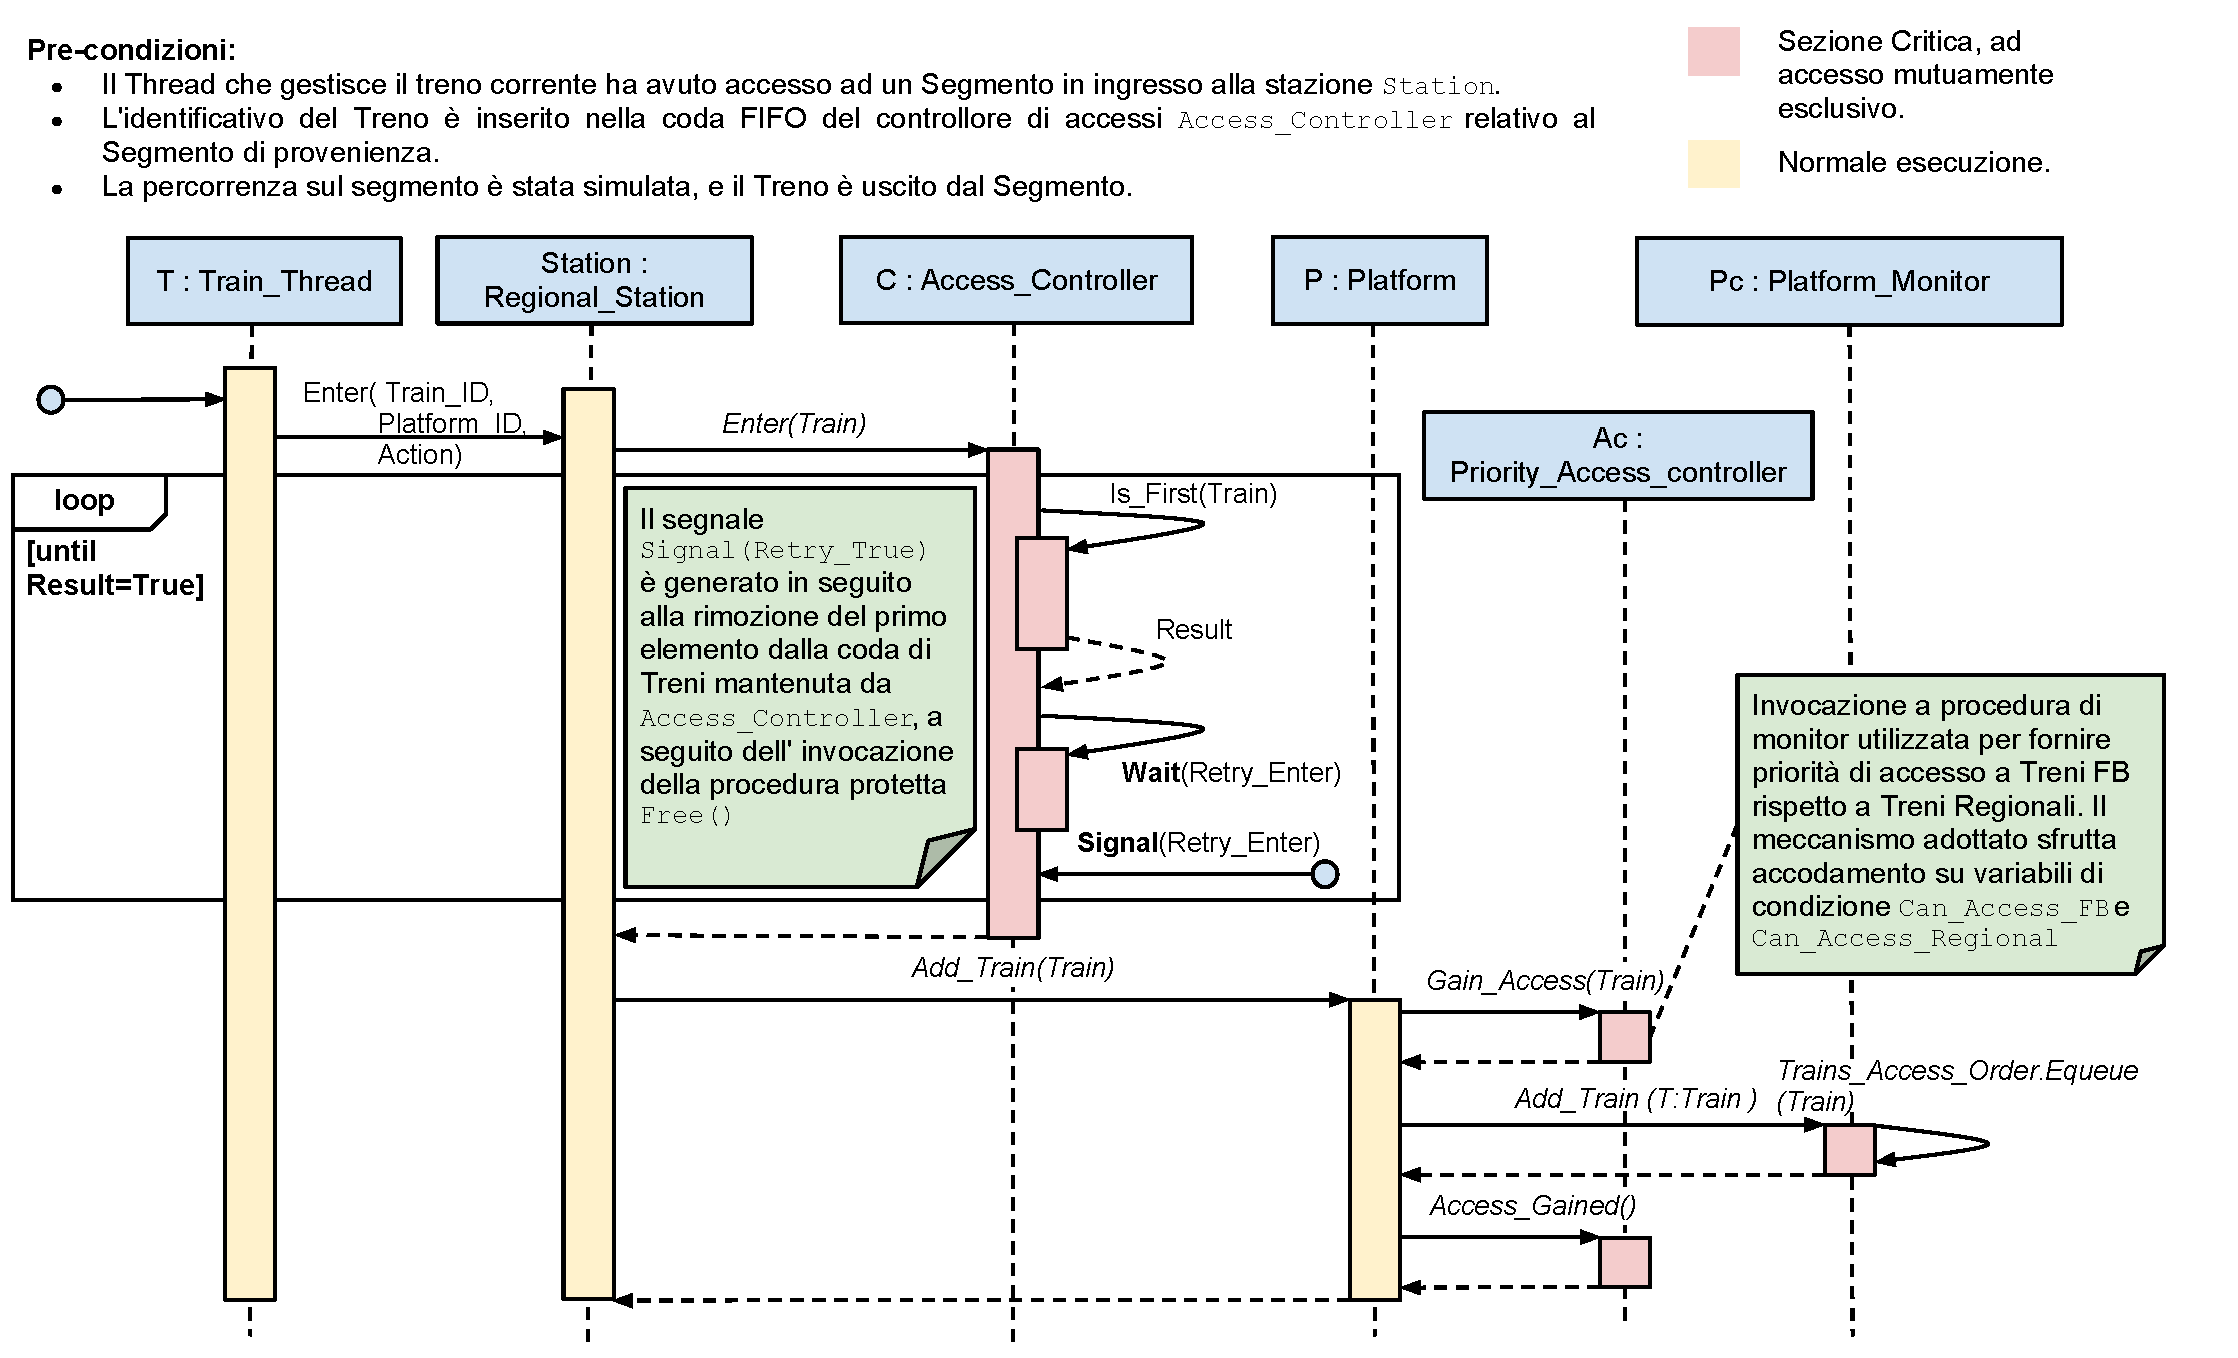
\includegraphics[scale=0.27,trim=0mm 20mm 0mm 20mm]{imgs/platform_access_1}
			\caption{\scriptsize Ingresso in una \stazione (1).}
		\end{figure}
		
	}

	\newframe{Soluzione Adottata}{\nameref{sol_conc}}{Treno}{2}{
	
		\begin{figure}
			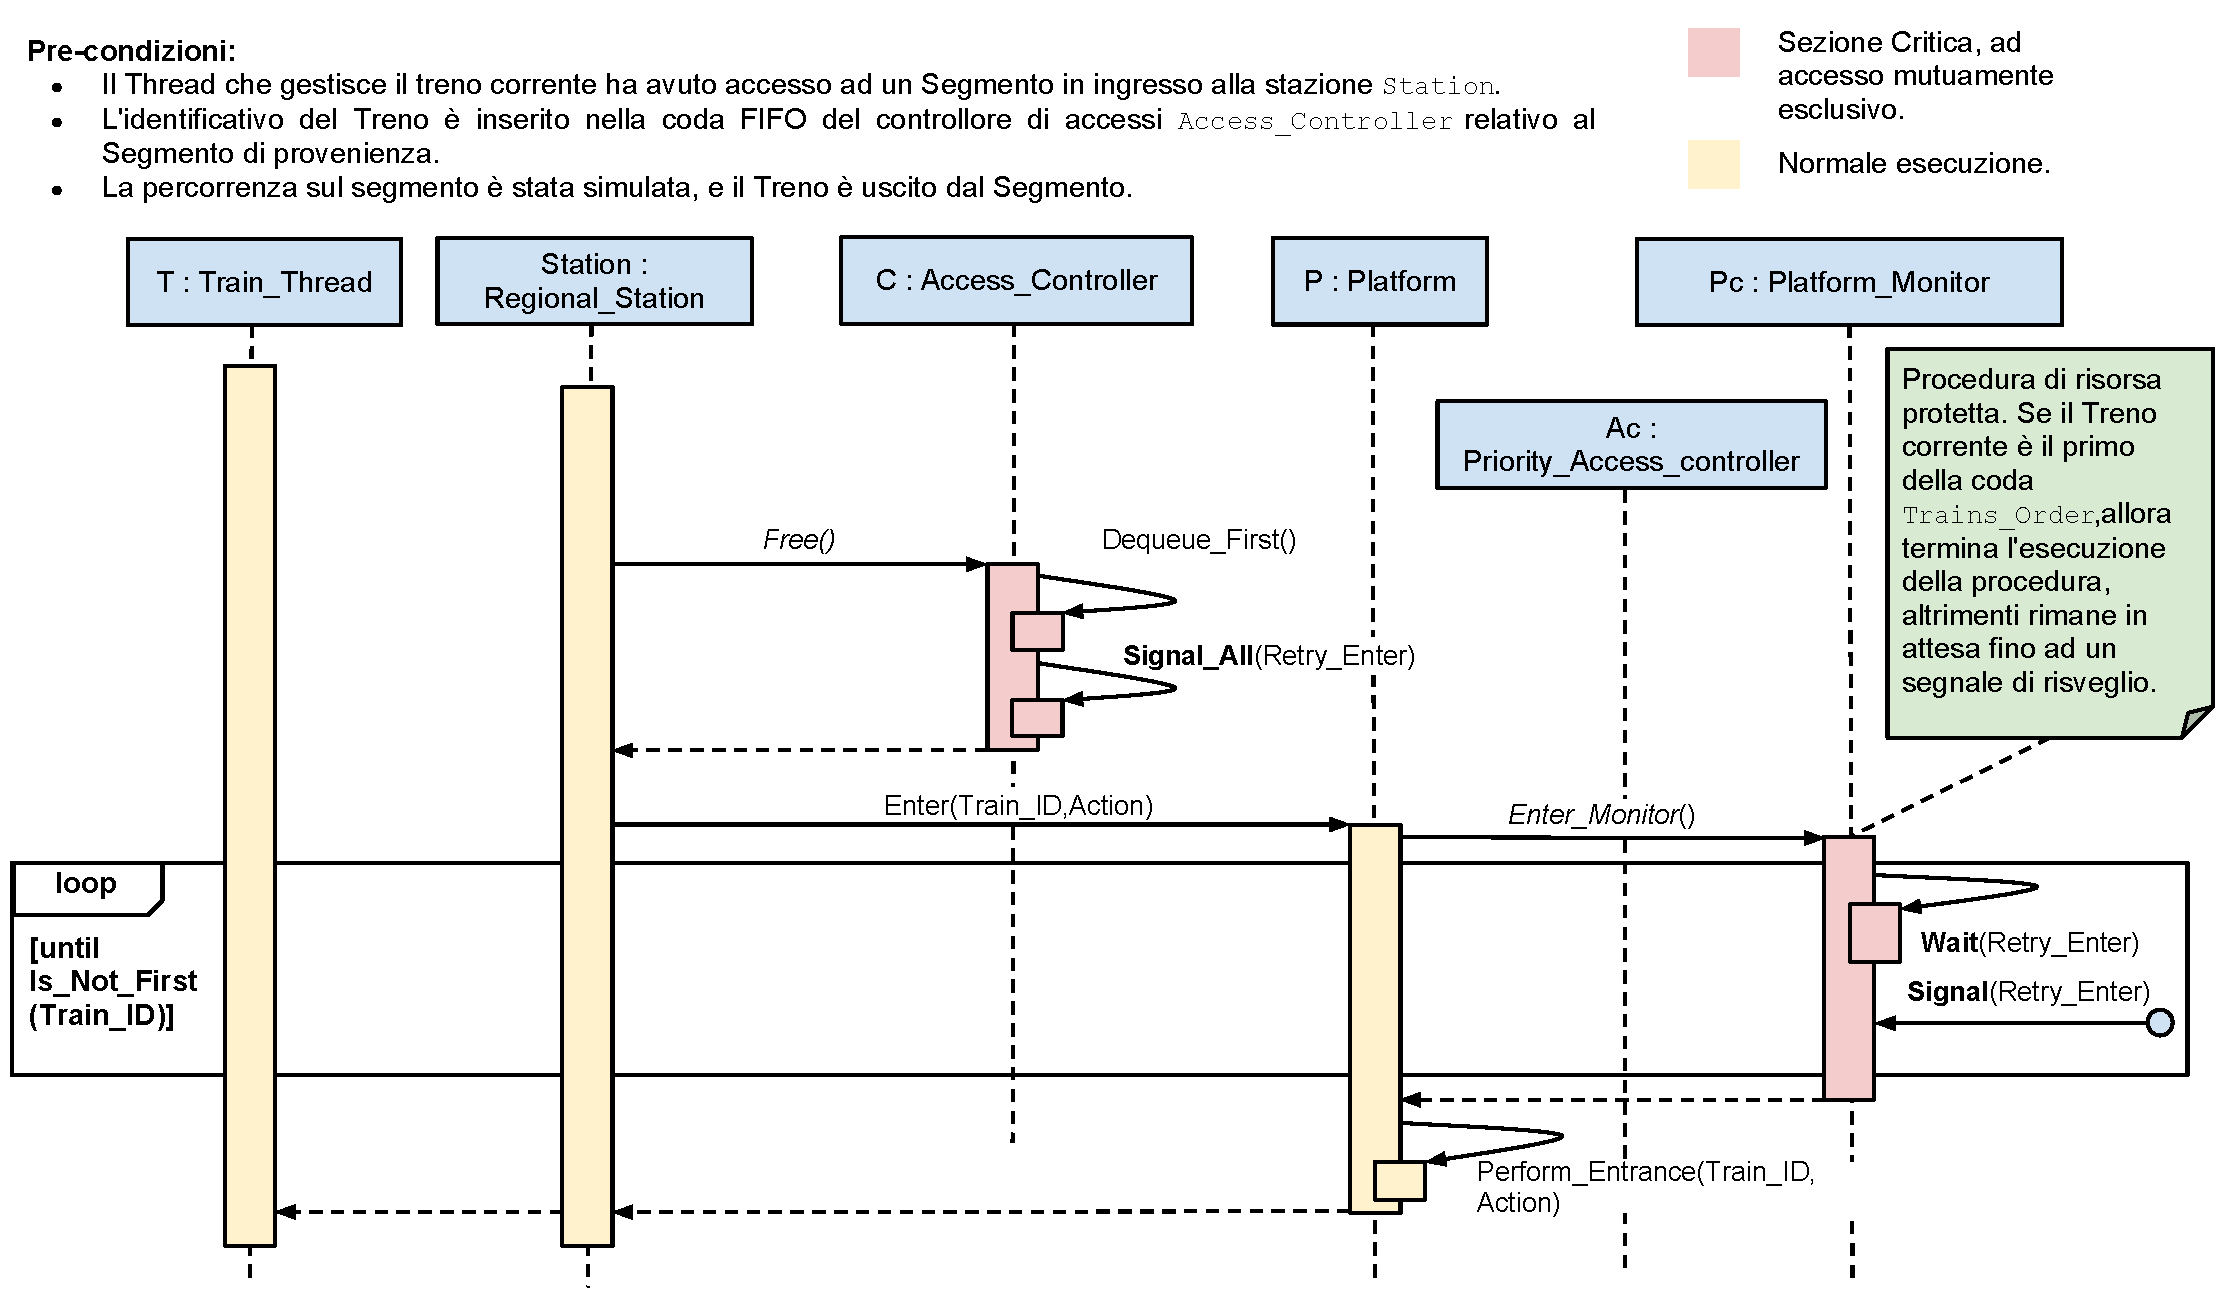
\includegraphics[scale=0.27,trim=0mm 20mm 0mm 20mm]{imgs/platform_access_2}
			\caption{\scriptsize Ingresso in una \stazione (2).}
		\end{figure}
		
	}

	\newframe{Soluzione Adottata}{\nameref{sol_conc}}{Treno}{3}{
	
		\begin{figure}
			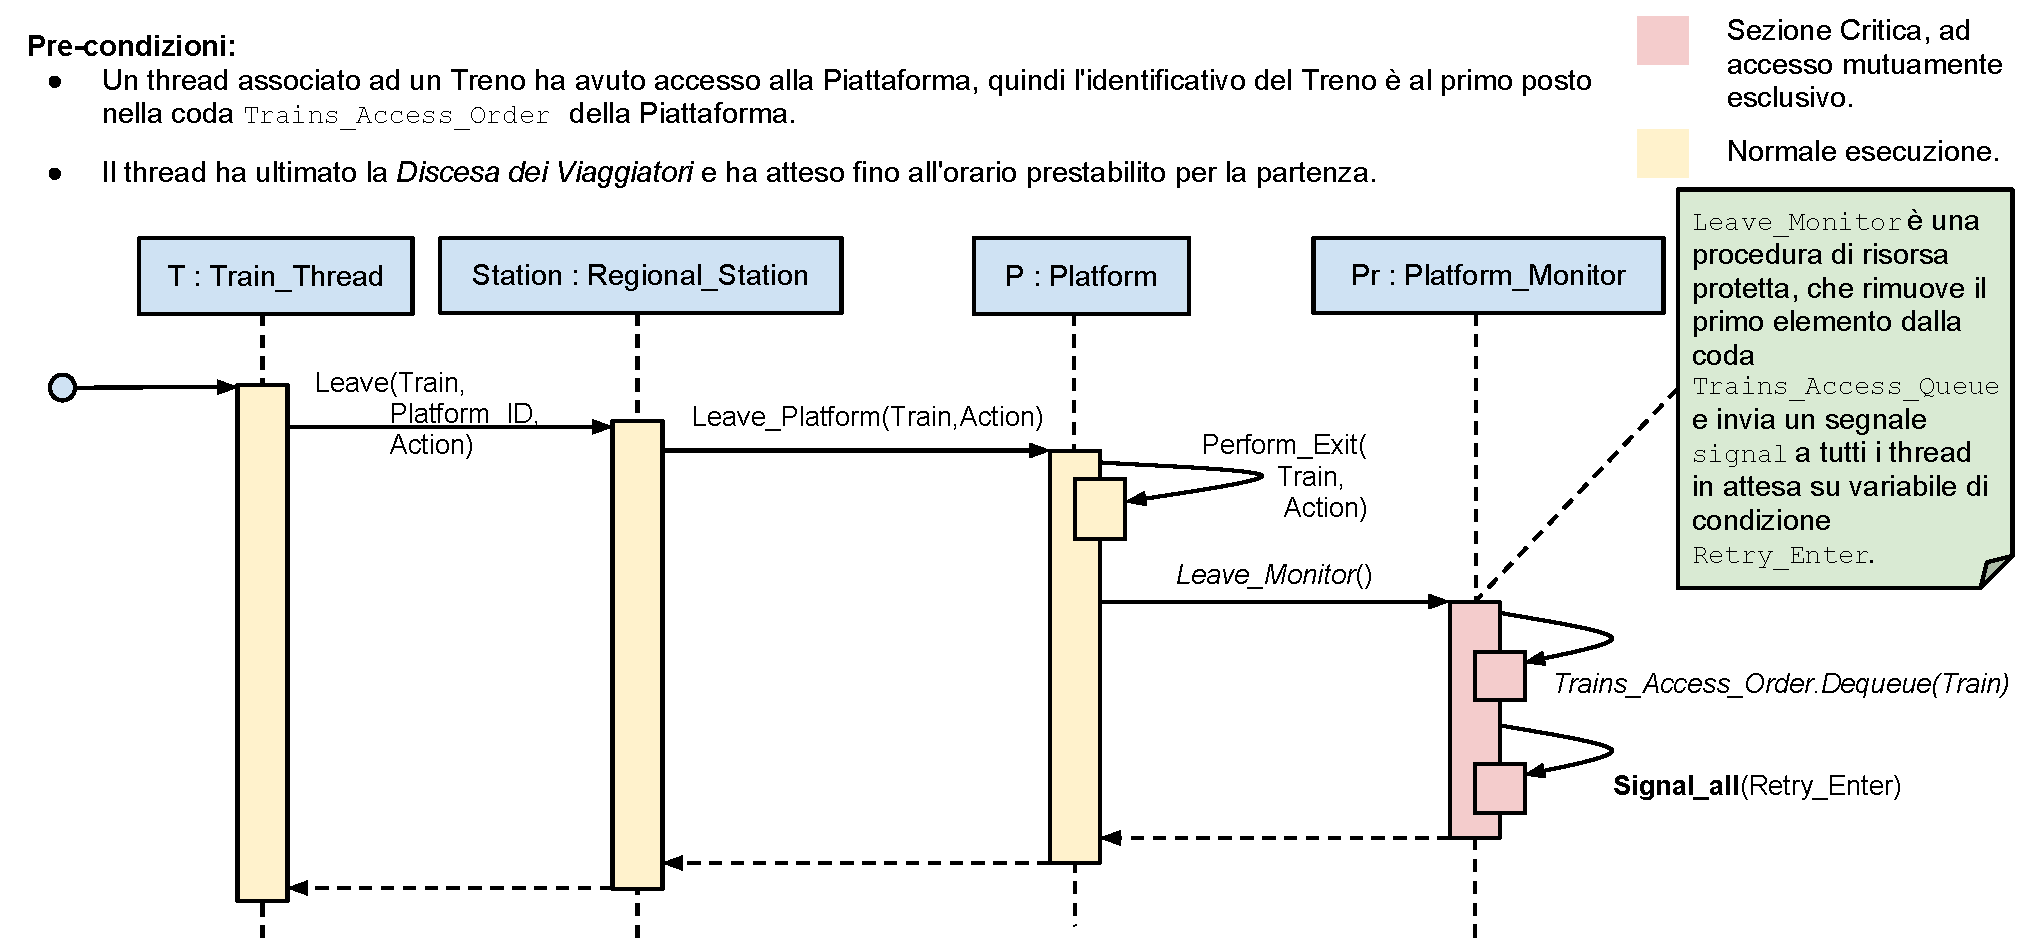
\includegraphics[scale=0.27,trim=0mm 0mm 0mm 0mm]{imgs/platform_exit}
			\caption{\scriptsize Uscita da una \piattaforma.}
		\end{figure}
		
	}

\end{document}

